% Options for packages loaded elsewhere
\PassOptionsToPackage{unicode}{hyperref}
\PassOptionsToPackage{hyphens}{url}
\PassOptionsToPackage{dvipsnames,svgnames,x11names}{xcolor}
%
\documentclass[
  letterpaper,
  DIV=11,
  numbers=noendperiod]{scrartcl}

\usepackage{amsmath,amssymb}
\usepackage{iftex}
\ifPDFTeX
  \usepackage[T1]{fontenc}
  \usepackage[utf8]{inputenc}
  \usepackage{textcomp} % provide euro and other symbols
\else % if luatex or xetex
  \usepackage{unicode-math}
  \defaultfontfeatures{Scale=MatchLowercase}
  \defaultfontfeatures[\rmfamily]{Ligatures=TeX,Scale=1}
\fi
\usepackage{lmodern}
\ifPDFTeX\else  
    % xetex/luatex font selection
\fi
% Use upquote if available, for straight quotes in verbatim environments
\IfFileExists{upquote.sty}{\usepackage{upquote}}{}
\IfFileExists{microtype.sty}{% use microtype if available
  \usepackage[]{microtype}
  \UseMicrotypeSet[protrusion]{basicmath} % disable protrusion for tt fonts
}{}
\makeatletter
\@ifundefined{KOMAClassName}{% if non-KOMA class
  \IfFileExists{parskip.sty}{%
    \usepackage{parskip}
  }{% else
    \setlength{\parindent}{0pt}
    \setlength{\parskip}{6pt plus 2pt minus 1pt}}
}{% if KOMA class
  \KOMAoptions{parskip=half}}
\makeatother
\usepackage{xcolor}
\setlength{\emergencystretch}{3em} % prevent overfull lines
\setcounter{secnumdepth}{-\maxdimen} % remove section numbering
% Make \paragraph and \subparagraph free-standing
\ifx\paragraph\undefined\else
  \let\oldparagraph\paragraph
  \renewcommand{\paragraph}[1]{\oldparagraph{#1}\mbox{}}
\fi
\ifx\subparagraph\undefined\else
  \let\oldsubparagraph\subparagraph
  \renewcommand{\subparagraph}[1]{\oldsubparagraph{#1}\mbox{}}
\fi


\providecommand{\tightlist}{%
  \setlength{\itemsep}{0pt}\setlength{\parskip}{0pt}}\usepackage{longtable,booktabs,array}
\usepackage{calc} % for calculating minipage widths
% Correct order of tables after \paragraph or \subparagraph
\usepackage{etoolbox}
\makeatletter
\patchcmd\longtable{\par}{\if@noskipsec\mbox{}\fi\par}{}{}
\makeatother
% Allow footnotes in longtable head/foot
\IfFileExists{footnotehyper.sty}{\usepackage{footnotehyper}}{\usepackage{footnote}}
\makesavenoteenv{longtable}
\usepackage{graphicx}
\makeatletter
\def\maxwidth{\ifdim\Gin@nat@width>\linewidth\linewidth\else\Gin@nat@width\fi}
\def\maxheight{\ifdim\Gin@nat@height>\textheight\textheight\else\Gin@nat@height\fi}
\makeatother
% Scale images if necessary, so that they will not overflow the page
% margins by default, and it is still possible to overwrite the defaults
% using explicit options in \includegraphics[width, height, ...]{}
\setkeys{Gin}{width=\maxwidth,height=\maxheight,keepaspectratio}
% Set default figure placement to htbp
\makeatletter
\def\fps@figure{htbp}
\makeatother

\KOMAoption{captions}{tableheading}
\makeatletter
\makeatother
\makeatletter
\makeatother
\makeatletter
\@ifpackageloaded{caption}{}{\usepackage{caption}}
\AtBeginDocument{%
\ifdefined\contentsname
  \renewcommand*\contentsname{Table of contents}
\else
  \newcommand\contentsname{Table of contents}
\fi
\ifdefined\listfigurename
  \renewcommand*\listfigurename{List of Figures}
\else
  \newcommand\listfigurename{List of Figures}
\fi
\ifdefined\listtablename
  \renewcommand*\listtablename{List of Tables}
\else
  \newcommand\listtablename{List of Tables}
\fi
\ifdefined\figurename
  \renewcommand*\figurename{Figure}
\else
  \newcommand\figurename{Figure}
\fi
\ifdefined\tablename
  \renewcommand*\tablename{Table}
\else
  \newcommand\tablename{Table}
\fi
}
\@ifpackageloaded{float}{}{\usepackage{float}}
\floatstyle{ruled}
\@ifundefined{c@chapter}{\newfloat{codelisting}{h}{lop}}{\newfloat{codelisting}{h}{lop}[chapter]}
\floatname{codelisting}{Listing}
\newcommand*\listoflistings{\listof{codelisting}{List of Listings}}
\makeatother
\makeatletter
\@ifpackageloaded{caption}{}{\usepackage{caption}}
\@ifpackageloaded{subcaption}{}{\usepackage{subcaption}}
\makeatother
\makeatletter
\@ifpackageloaded{tcolorbox}{}{\usepackage[skins,breakable]{tcolorbox}}
\makeatother
\makeatletter
\@ifundefined{shadecolor}{\definecolor{shadecolor}{rgb}{.97, .97, .97}}
\makeatother
\makeatletter
\makeatother
\makeatletter
\makeatother
\ifLuaTeX
  \usepackage{selnolig}  % disable illegal ligatures
\fi
\IfFileExists{bookmark.sty}{\usepackage{bookmark}}{\usepackage{hyperref}}
\IfFileExists{xurl.sty}{\usepackage{xurl}}{} % add URL line breaks if available
\urlstyle{same} % disable monospaced font for URLs
\hypersetup{
  colorlinks=true,
  linkcolor={blue},
  filecolor={Maroon},
  citecolor={Blue},
  urlcolor={Blue},
  pdfcreator={LaTeX via pandoc}}

\author{}
\date{}

\begin{document}
\ifdefined\Shaded\renewenvironment{Shaded}{\begin{tcolorbox}[breakable, interior hidden, enhanced, borderline west={3pt}{0pt}{shadecolor}, frame hidden, sharp corners, boxrule=0pt]}{\end{tcolorbox}}\fi

\hypertarget{results}{%
\section{Results}\label{results}}

\hypertarget{perceptions-of-wildlife-health-importance}{%
\subsubsection{Perceptions of wildlife health
importance}\label{perceptions-of-wildlife-health-importance}}

\hypertarget{appendix-s2.-level-of-agreement-grey-scale-among-non-local-protected-area-data-managers-with-the-statements-pathogens-carried-by-wildlife-inhabiting-the-protected-areas-where-i-work-in-can-affect-livestock-health.-brown-pathogens-carried-by-wildlife-inhabiting-the-protected-areas-where-i-work-in-can-affect-human-health.-red-human-or-livestock-pathogens-can-affect-wildlife-populations-inhabiting-the-protected-areas-where-i-work-in.-blue-and-wildlife-health-is-important-to-achieve-the-conservation-goals-of-the-protected-areas-where-i-work-green.-overall-frequency-of-encounters-with-sick-and-injured-wildlife-was-requested-in-a-unique-question-therefore-rows-one-and-two-show-the-same-total-number-of-responses-per-encounter-category.}{%
\paragraph{Appendix S2. Level of agreement (grey scale) among non-local
protected area data managers with the statements ``Pathogens carried by
wildlife inhabiting the protected area(s) where I work in can affect
livestock health.'' (brown), ``Pathogens carried by wildlife inhabiting
the protected area(s) where I work in can affect human health.'' (red),
``Human or livestock pathogens can affect wildlife populations
inhabiting the protected area(s) where I work in.'' (blue), and
``Wildlife health is important to achieve the conservation goals of the
protected area(s) where I work,'' (green). Overall frequency of
encounters with sick and injured wildlife was requested in a unique
question; therefore, rows one and two show the same total number of
responses per encounter
category.}\label{appendix-s2.-level-of-agreement-grey-scale-among-non-local-protected-area-data-managers-with-the-statements-pathogens-carried-by-wildlife-inhabiting-the-protected-areas-where-i-work-in-can-affect-livestock-health.-brown-pathogens-carried-by-wildlife-inhabiting-the-protected-areas-where-i-work-in-can-affect-human-health.-red-human-or-livestock-pathogens-can-affect-wildlife-populations-inhabiting-the-protected-areas-where-i-work-in.-blue-and-wildlife-health-is-important-to-achieve-the-conservation-goals-of-the-protected-areas-where-i-work-green.-overall-frequency-of-encounters-with-sick-and-injured-wildlife-was-requested-in-a-unique-question-therefore-rows-one-and-two-show-the-same-total-number-of-responses-per-encounter-category.}}

\begin{figure}[H]

{\centering 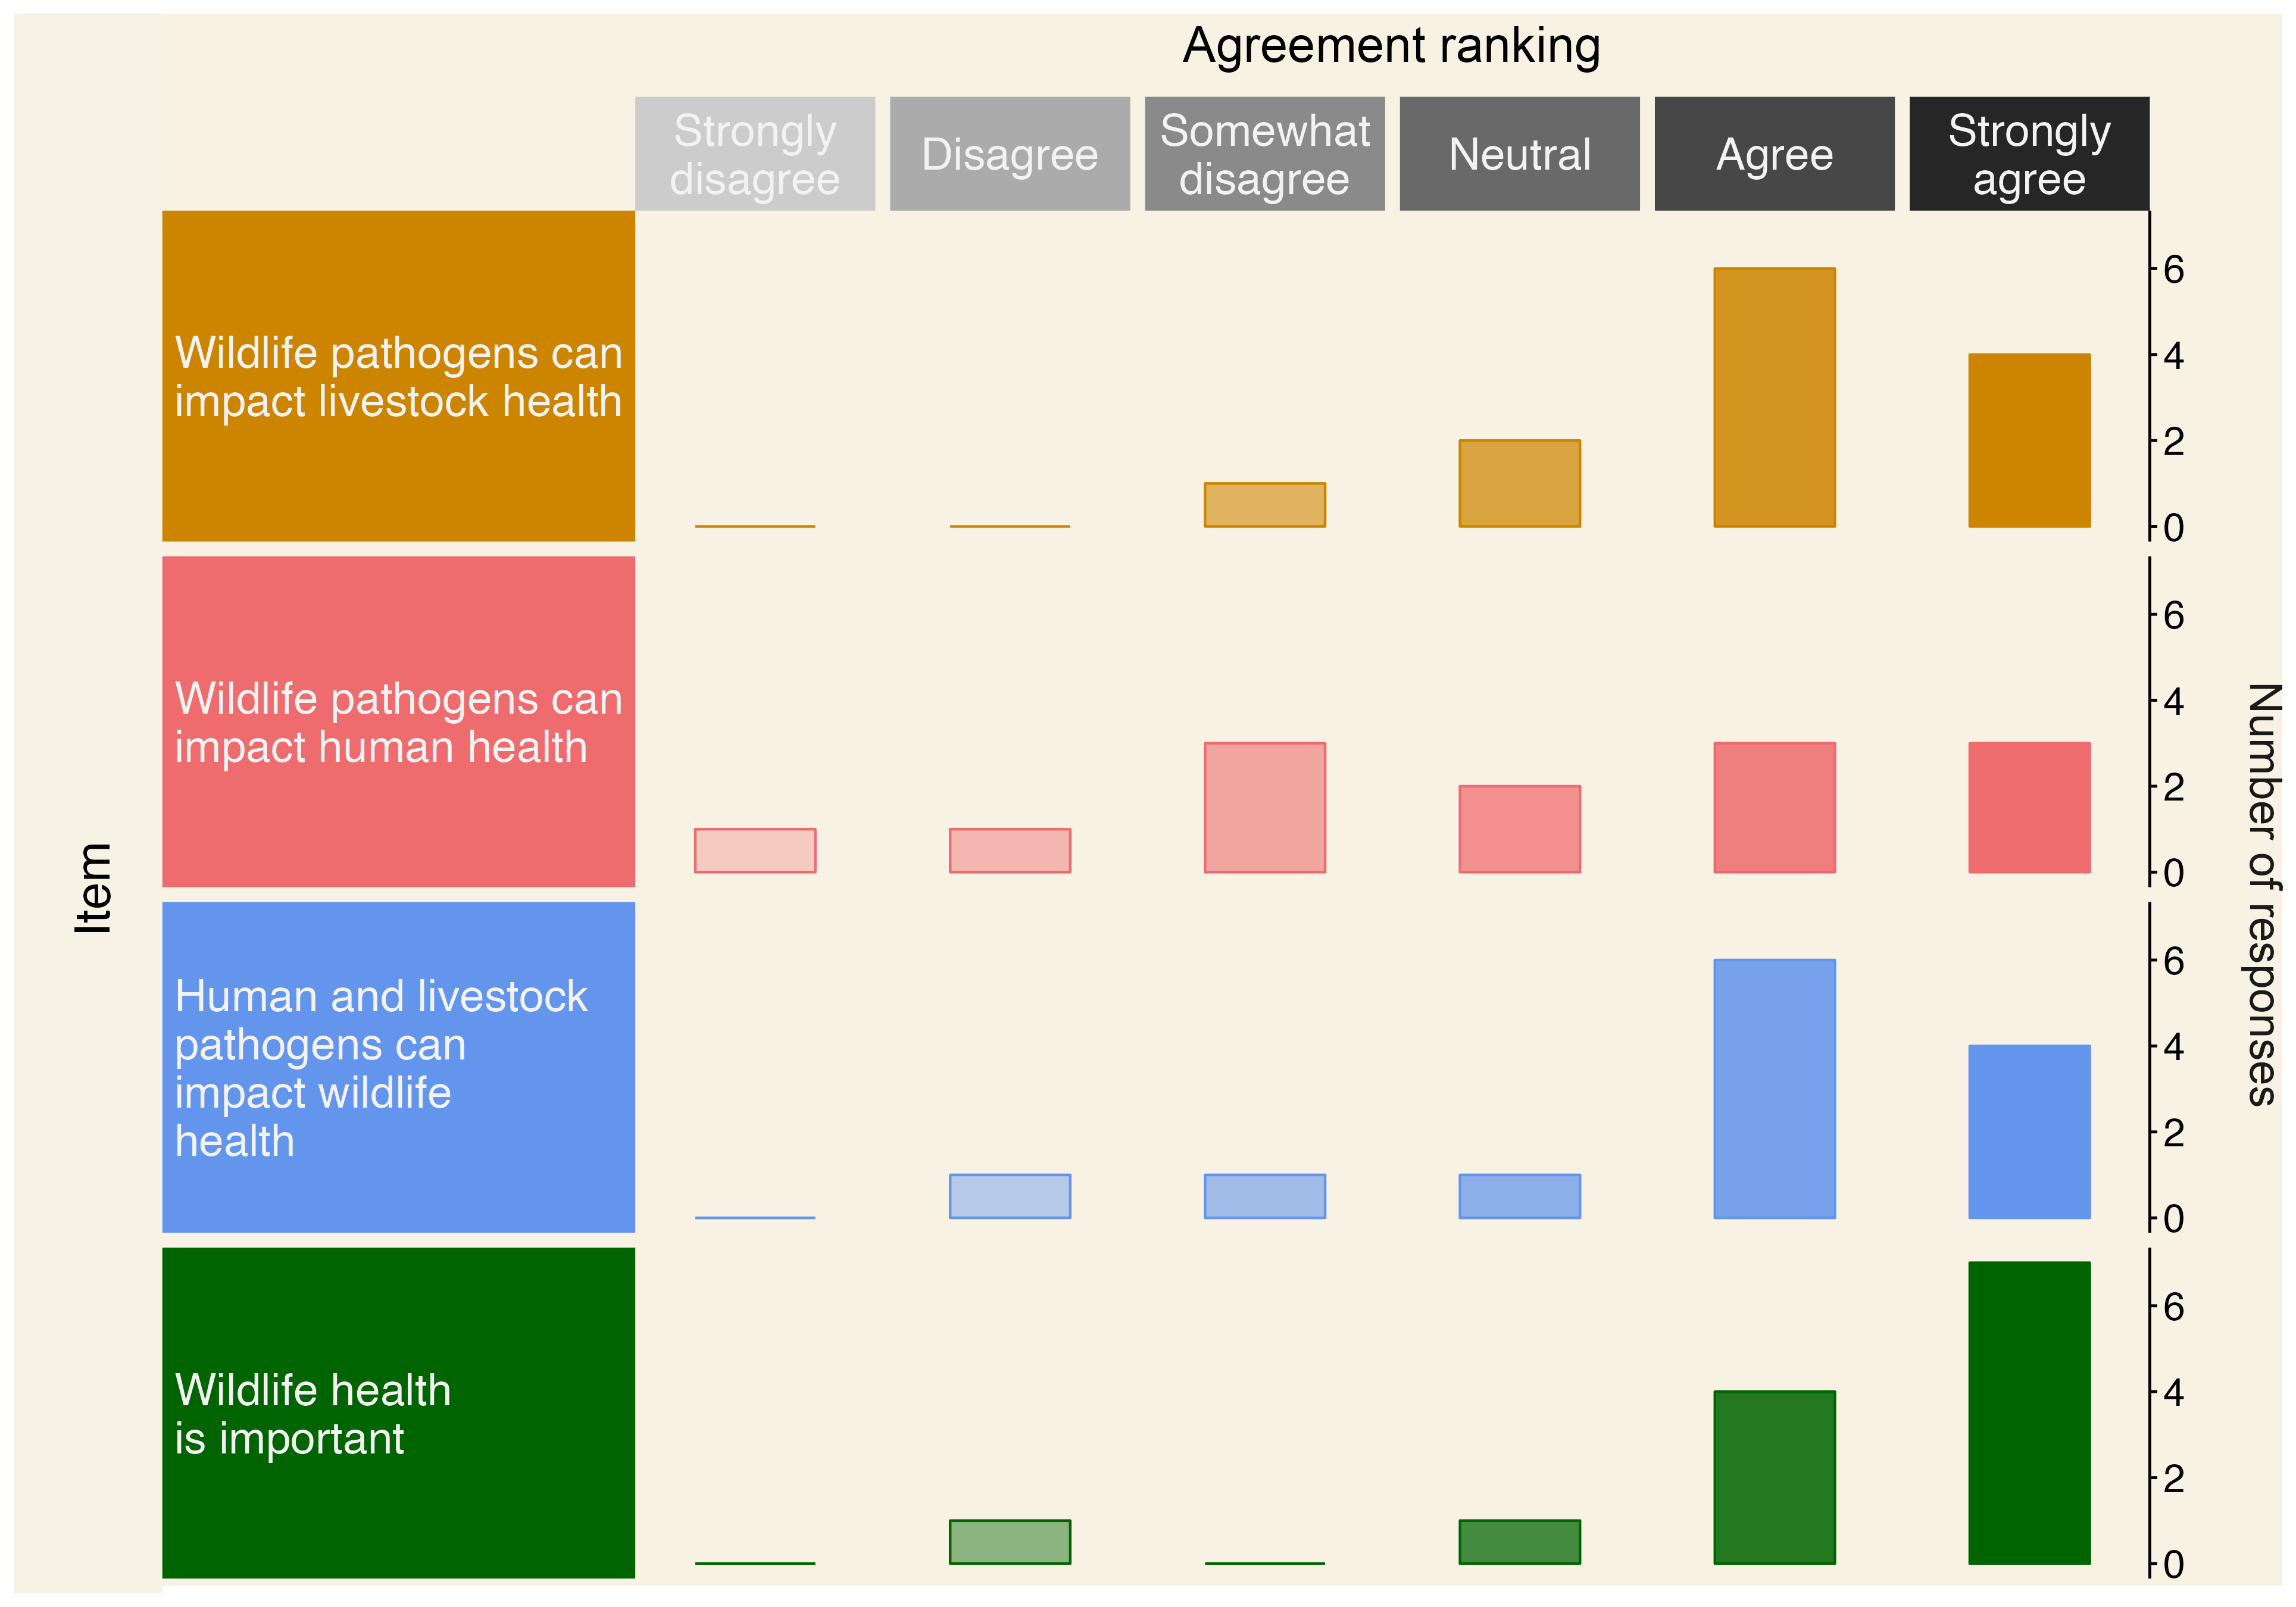
\includegraphics[width=6.25in,height=\textheight]{plots/appedix_plot_1.png}

}

\end{figure}

\hypertarget{encounters-with-injured-sick-or-dead-wildlife-and-documentation}{%
\subsubsection{Encounters with injured, sick, or dead wildlife and
documentation}\label{encounters-with-injured-sick-or-dead-wildlife-and-documentation}}

\hypertarget{appendix-s3.-number-of-non-local-protected-area-data-managers-who-reported-that-the-health-status-of-and-frequency-of-encounters-with-wildlife-are-recorded-or-not-recorded-in-the-protected-area-they-worked-in.-green-bars-represent-the-proportion-of-respondents-that-reported-recording-of-wildlife-in-each-category.}{%
\paragraph{Appendix S3. Number of non-local protected area data managers
who reported that the health status of and frequency of encounters with
wildlife are recorded or not recorded in the protected area they worked
in. Green bars represent the proportion of respondents that reported
recording of wildlife in each
category.}\label{appendix-s3.-number-of-non-local-protected-area-data-managers-who-reported-that-the-health-status-of-and-frequency-of-encounters-with-wildlife-are-recorded-or-not-recorded-in-the-protected-area-they-worked-in.-green-bars-represent-the-proportion-of-respondents-that-reported-recording-of-wildlife-in-each-category.}}

\begin{figure}[H]

{\centering 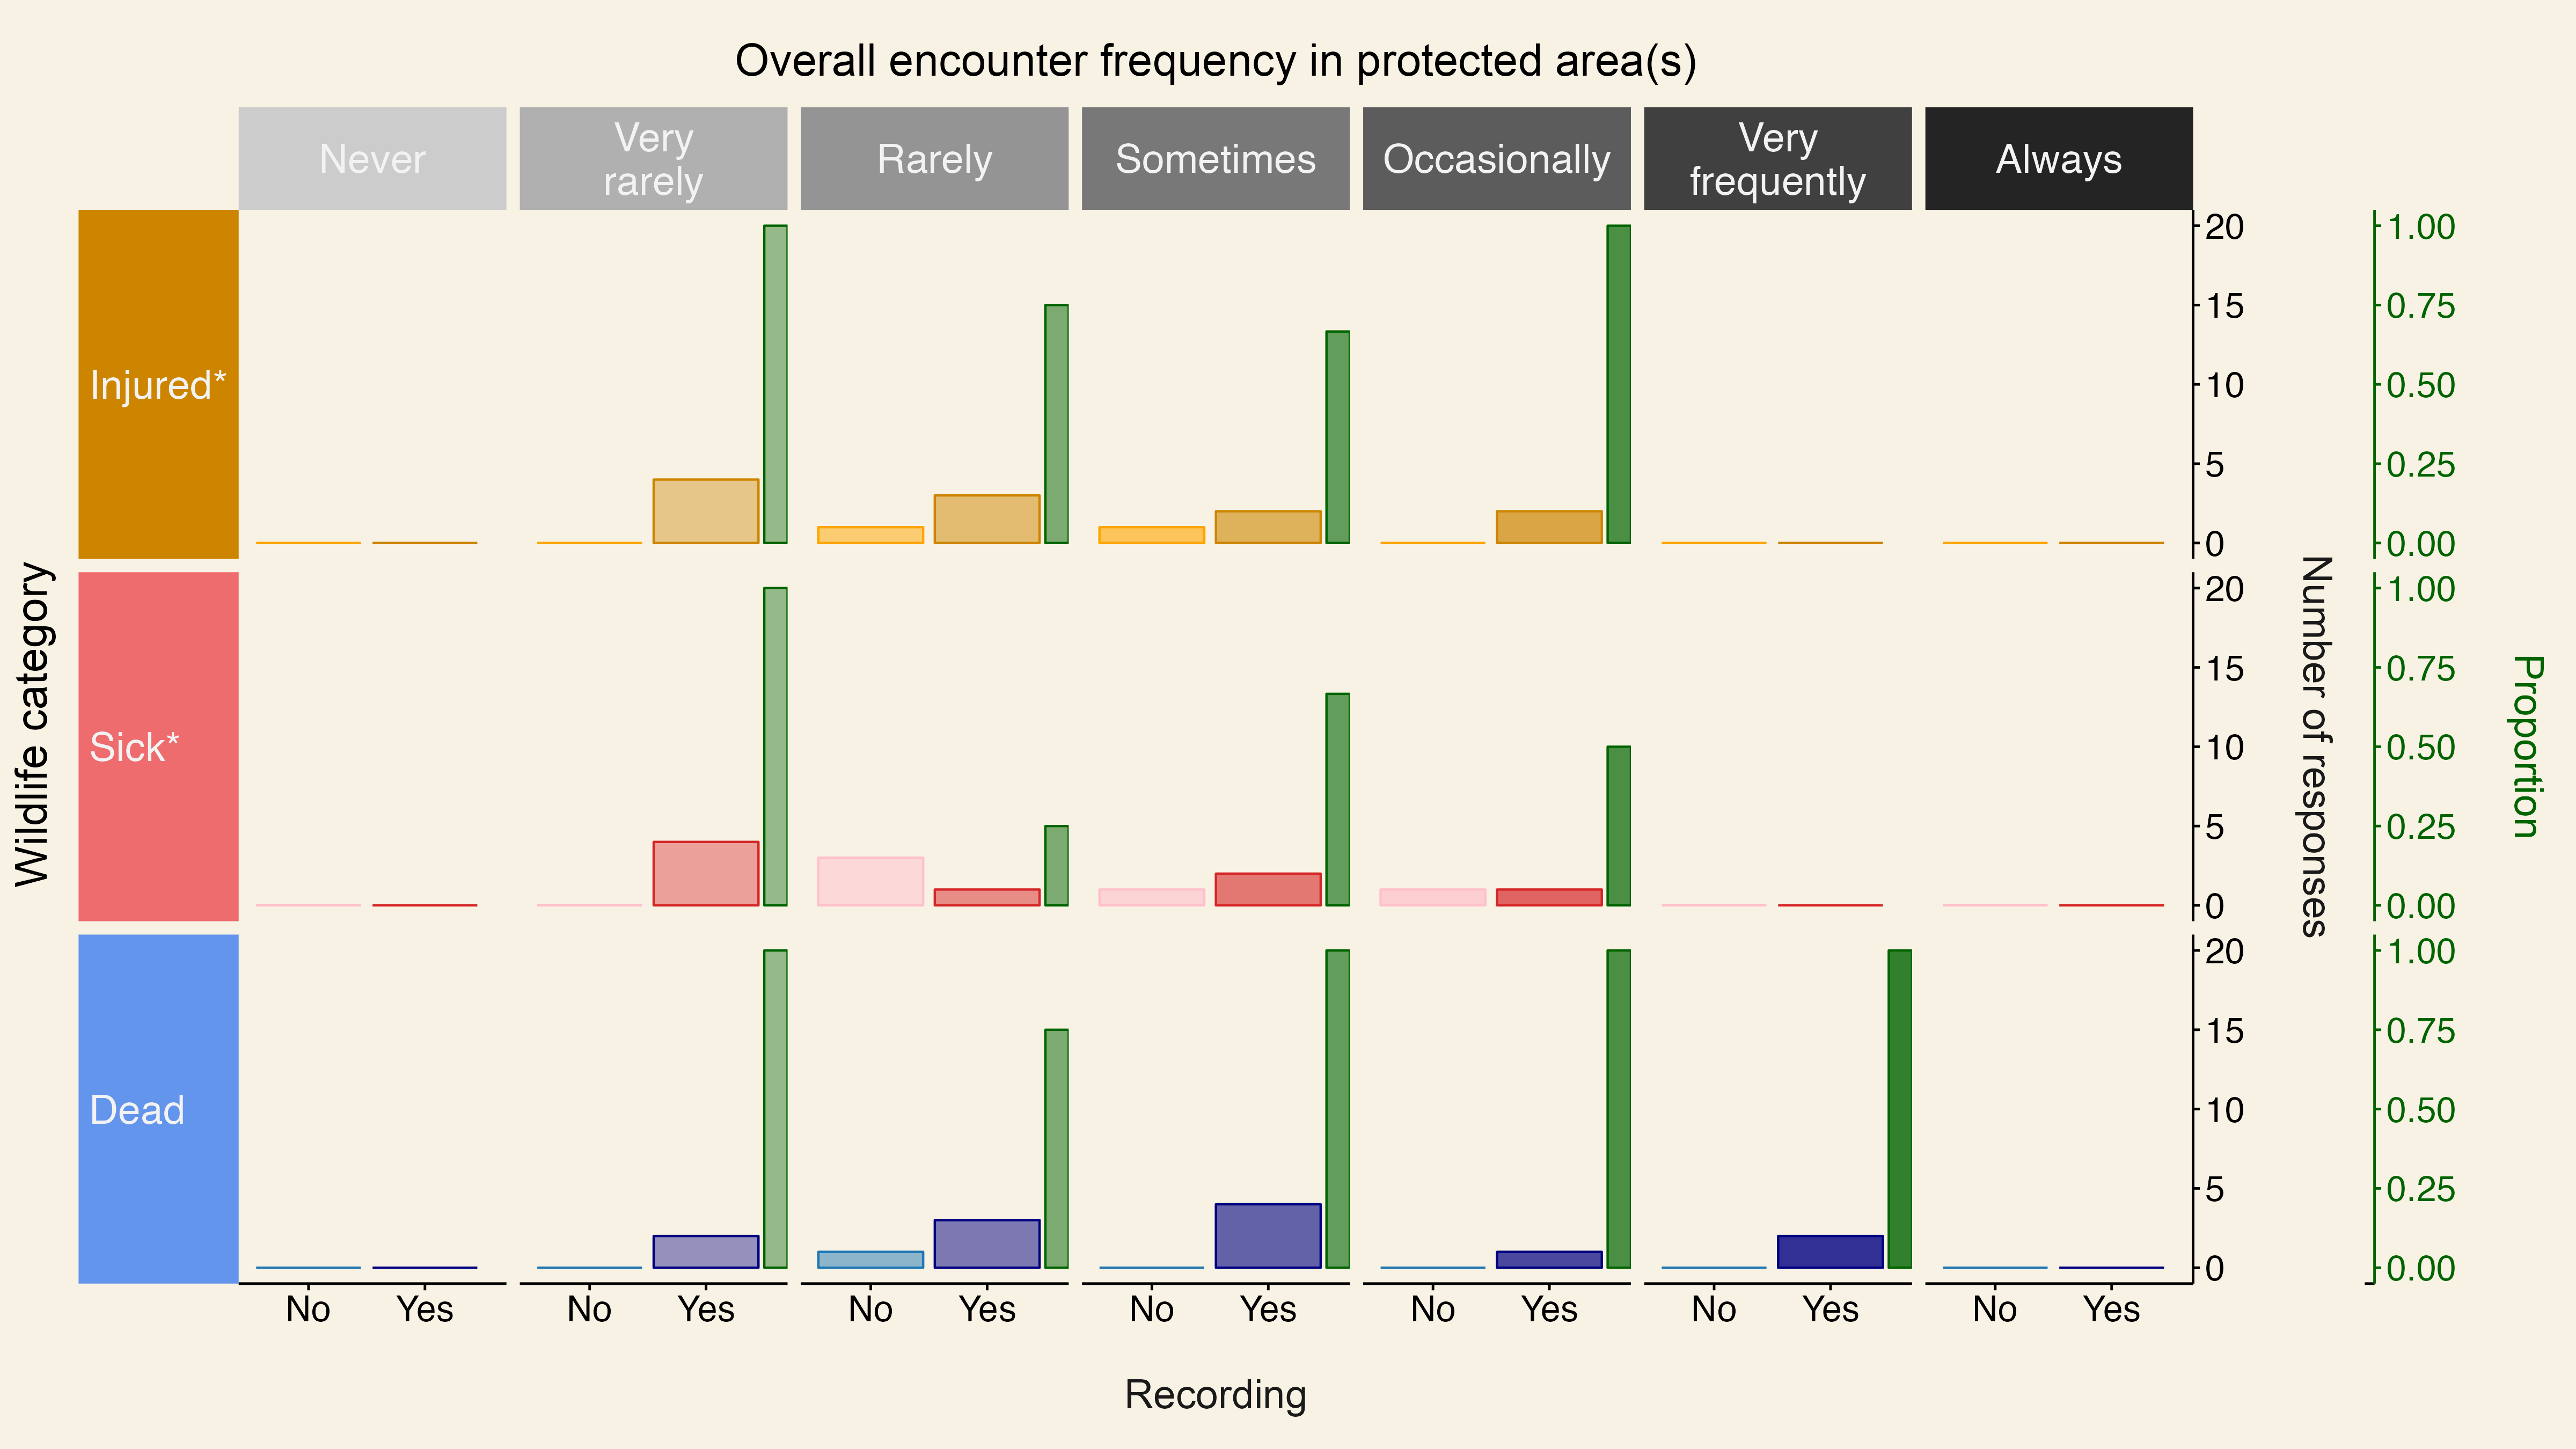
\includegraphics[width=6.25in,height=\textheight]{plots/appedix_plot_2.png}

}

\end{figure}

\newpage

\hypertarget{documentation-methods}{%
\subsubsection{Documentation methods}\label{documentation-methods}}

\hypertarget{appendix-s4.-distribution-of-the-methods-of-documentation-second-column-of-healthy-sick-injured-or-dead-wildlife-found-during-ranger-patrols-as-reported-by-non-local-protected-area-data-managers-and-the-recording-of-specific-types-of-data-for-each-wildlife-health-status-across-documentation-methods-black-line-50.}{%
\paragraph{Appendix S4. Distribution of the methods of documentation
(second column) of healthy, sick, injured, or dead wildlife found during
ranger patrols as reported by non-local protected area data managers and
the recording of specific types of data for each wildlife health status
across documentation methods (black line,
50\%).}\label{appendix-s4.-distribution-of-the-methods-of-documentation-second-column-of-healthy-sick-injured-or-dead-wildlife-found-during-ranger-patrols-as-reported-by-non-local-protected-area-data-managers-and-the-recording-of-specific-types-of-data-for-each-wildlife-health-status-across-documentation-methods-black-line-50.}}

\begin{figure}[H]

{\centering 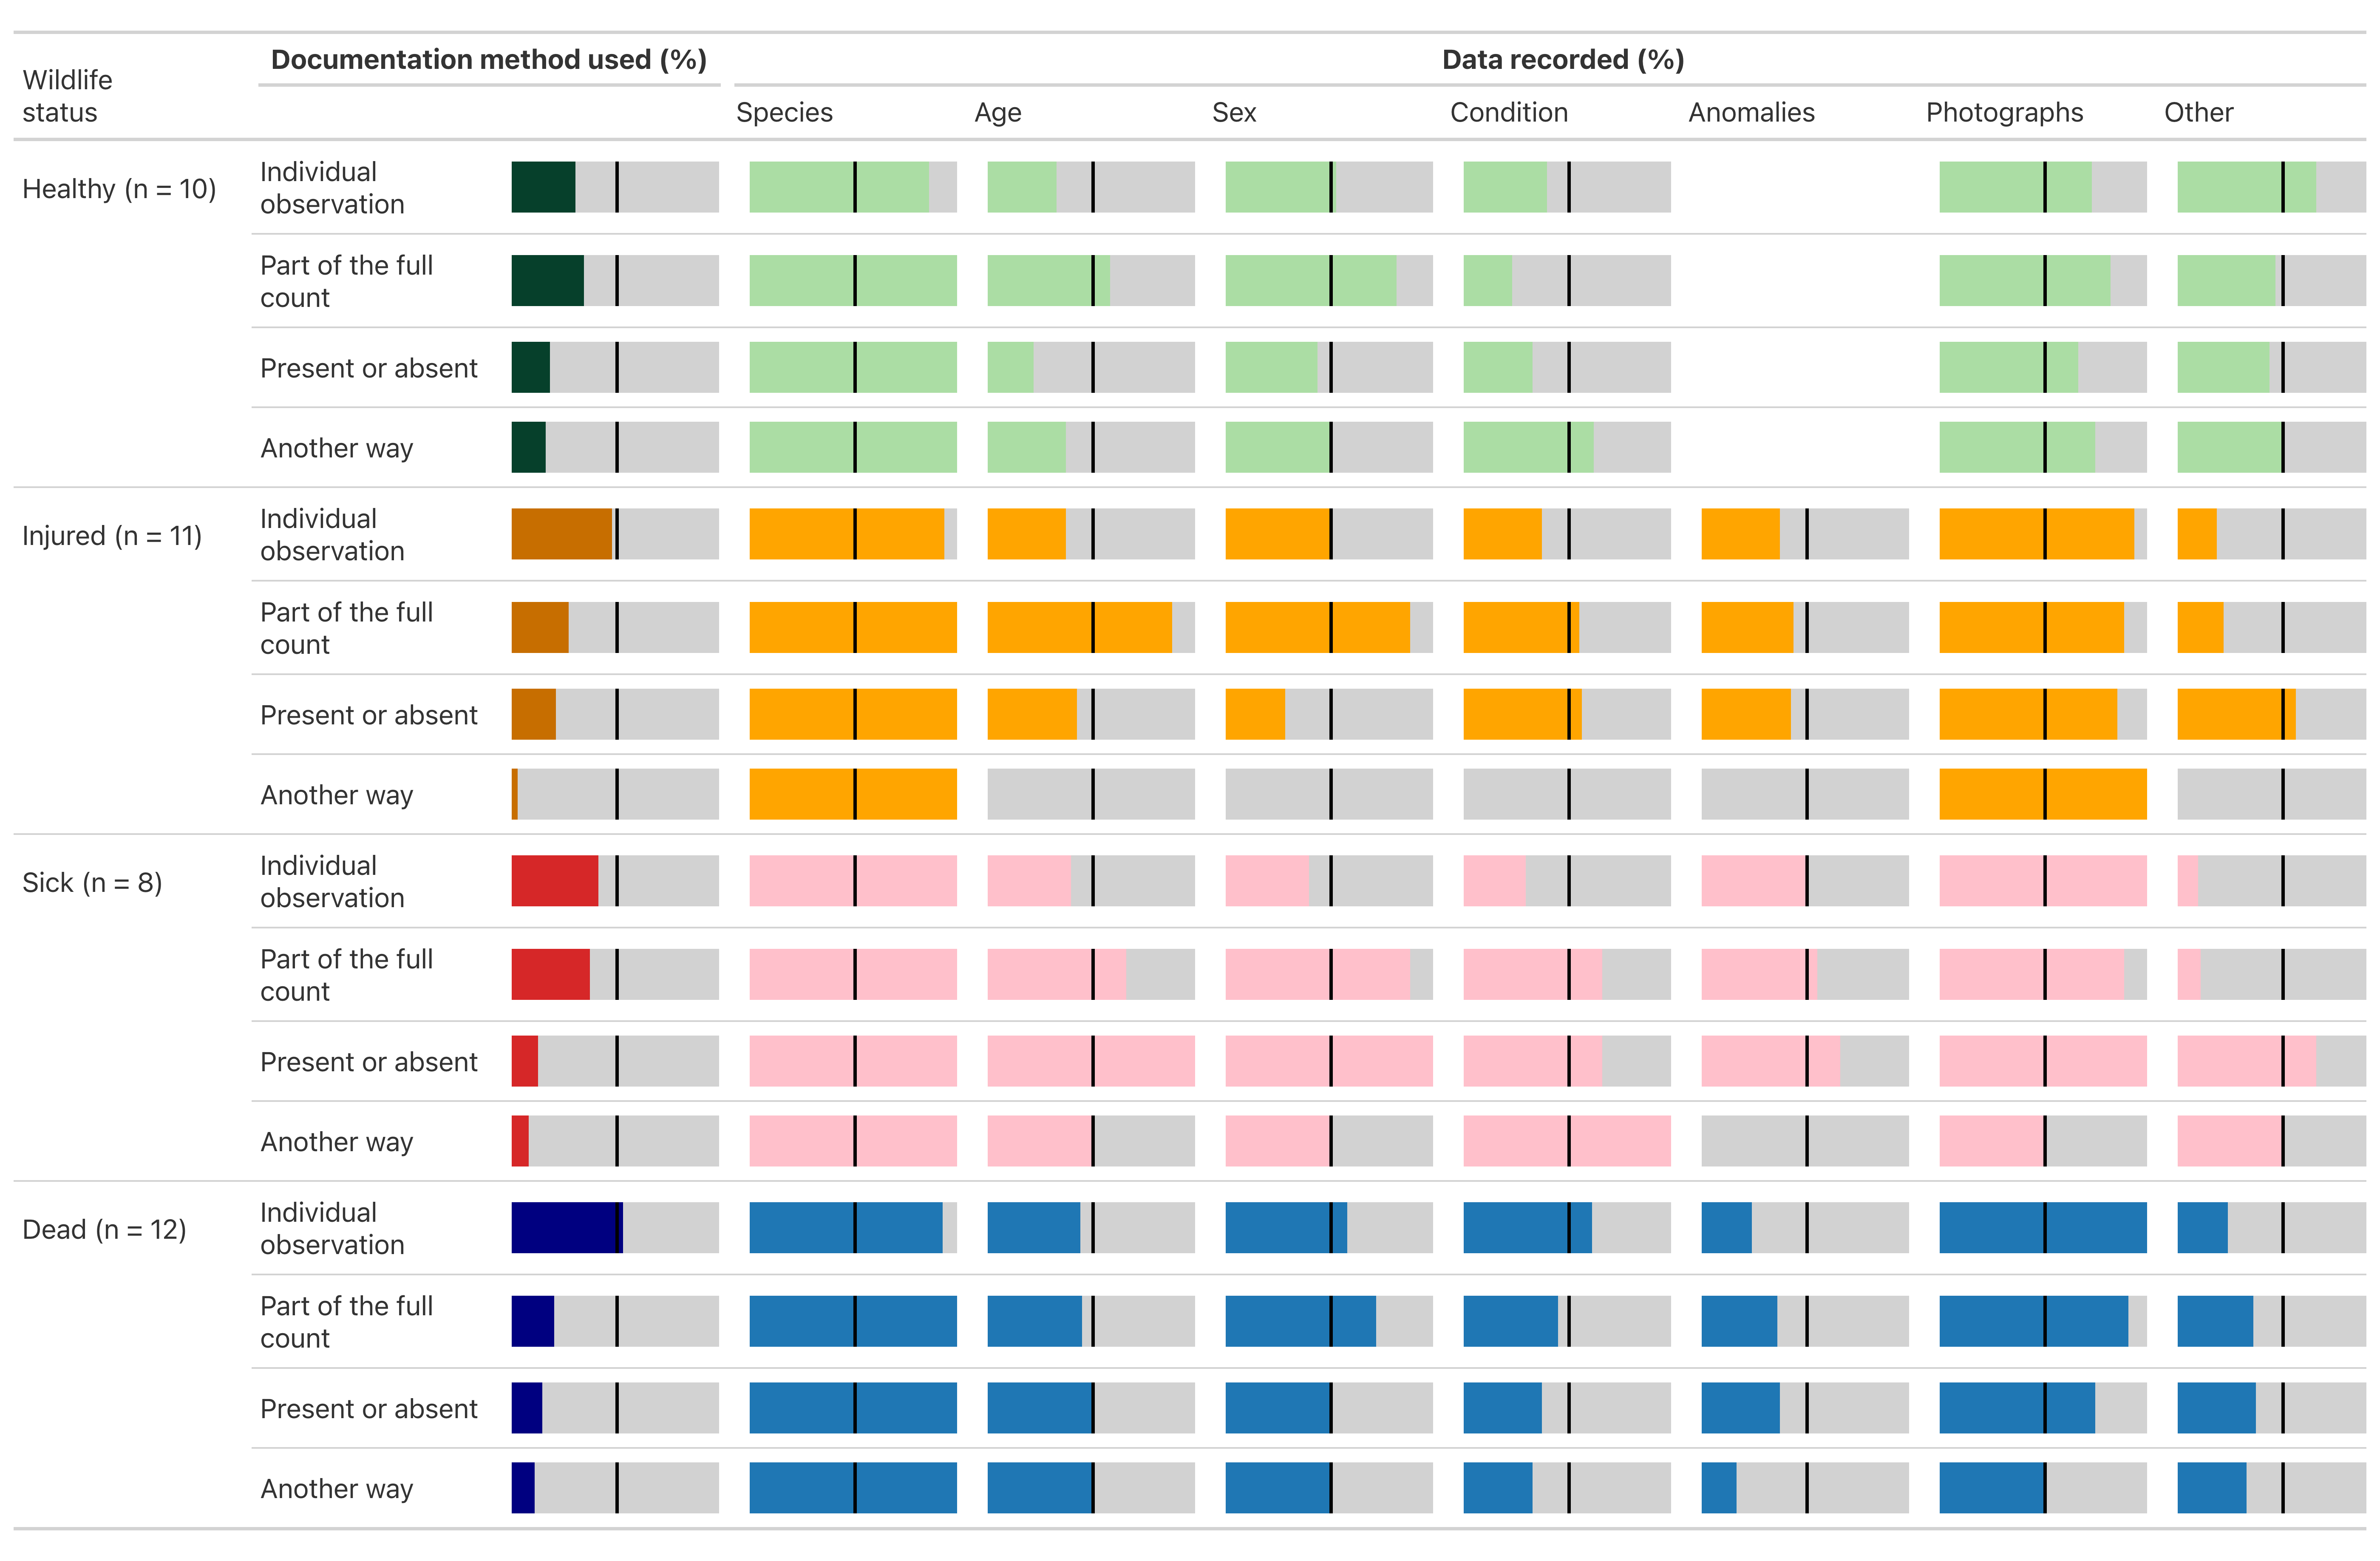
\includegraphics[width=6.25in,height=\textheight]{plots/appedix_plot_3.png}

}

\end{figure}

\newpage

\hypertarget{domestic-animals-in-protected-areas}{%
\subsubsection{Domestic animals in protected
areas}\label{domestic-animals-in-protected-areas}}

\hypertarget{appendix-s5.-responses-of-non-local-protected-area-data-manager-to-statements-that-the-presence-and-health-of-domestic-animals-in-protected-areas-is-a-conservation-concern-red-no-recording-of-domestic-animals-light-blue-recording-of-domestic-animals-but-not-their-health-status-dark-blue-recording-of-domestic-animals-and-their-health-status.-data-are-from-the-group-of-non-local-protected-area-data-managers-who-reported-the-presence-of-domestic-animals-in-the-protected-area.}{%
\paragraph{Appendix S5. Responses of non-local protected area data
manager to statements that the presence and health of domestic animals
in protected areas is a conservation concern (red, no recording of
domestic animals; light blue, recording of domestic animals but not
their health status; dark blue, recording of domestic animals and their
health status). Data are from the group of non-local protected area data
managers who reported the presence of domestic animals in the protected
area.}\label{appendix-s5.-responses-of-non-local-protected-area-data-manager-to-statements-that-the-presence-and-health-of-domestic-animals-in-protected-areas-is-a-conservation-concern-red-no-recording-of-domestic-animals-light-blue-recording-of-domestic-animals-but-not-their-health-status-dark-blue-recording-of-domestic-animals-and-their-health-status.-data-are-from-the-group-of-non-local-protected-area-data-managers-who-reported-the-presence-of-domestic-animals-in-the-protected-area.}}

\begin{figure}[H]

{\centering 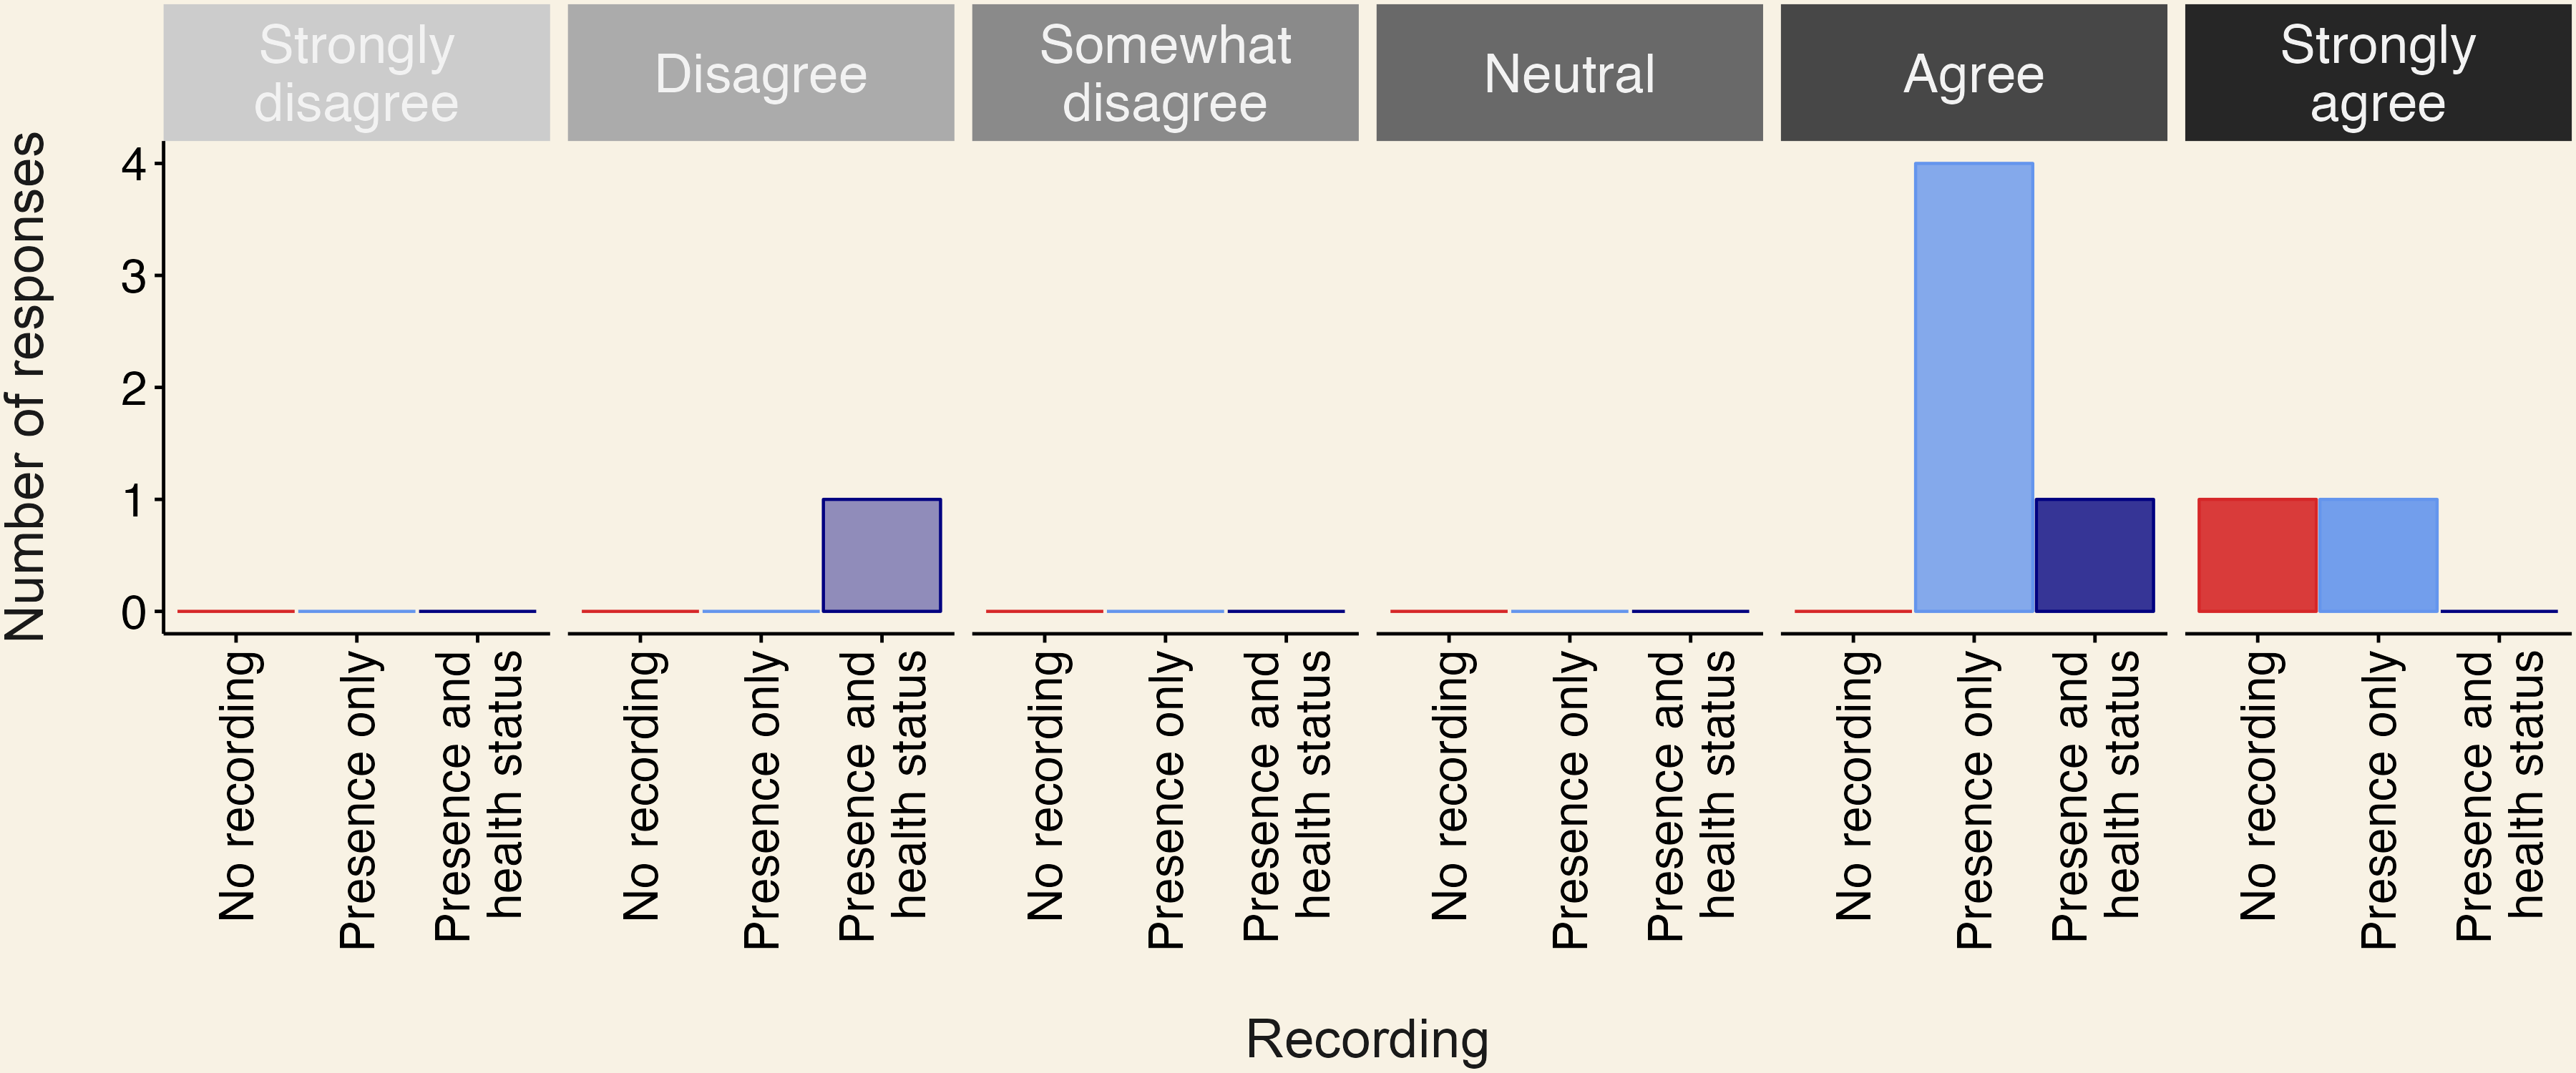
\includegraphics[width=6.25in,height=\textheight]{plots/appedix_plot_4.png}

}

\end{figure}

\newpage

\hypertarget{discussion}{%
\section{Discussion}\label{discussion}}

\hypertarget{appendix-s6.-distribution-of-protected-area-data-managers-responses-local-and-non-local-across-their-overall-agreement-with-the-statements-human-and-livestock-pathogens-can-impact-wildlife-health-and-introduced-domestic-animals-are-a-concern-for-the-conservation-goals-of-the-protected-area-for-those-protected-area-managers-local-and-non-local-that-reported-the-absence-of-domestic-animals-in-the-protected-area.}{%
\paragraph{Appendix S6. Distribution of protected area data managers
responses (local and non-local) across their overall agreement with the
statements ``Human and livestock pathogens can impact wildlife health''
and ``Introduced domestic animals are a concern for the conservation
goals of the protected area'' for those protected area managers (local
and non-local) that reported the absence of domestic animals in the
protected
area.}\label{appendix-s6.-distribution-of-protected-area-data-managers-responses-local-and-non-local-across-their-overall-agreement-with-the-statements-human-and-livestock-pathogens-can-impact-wildlife-health-and-introduced-domestic-animals-are-a-concern-for-the-conservation-goals-of-the-protected-area-for-those-protected-area-managers-local-and-non-local-that-reported-the-absence-of-domestic-animals-in-the-protected-area.}}

\begin{figure}[H]

{\centering 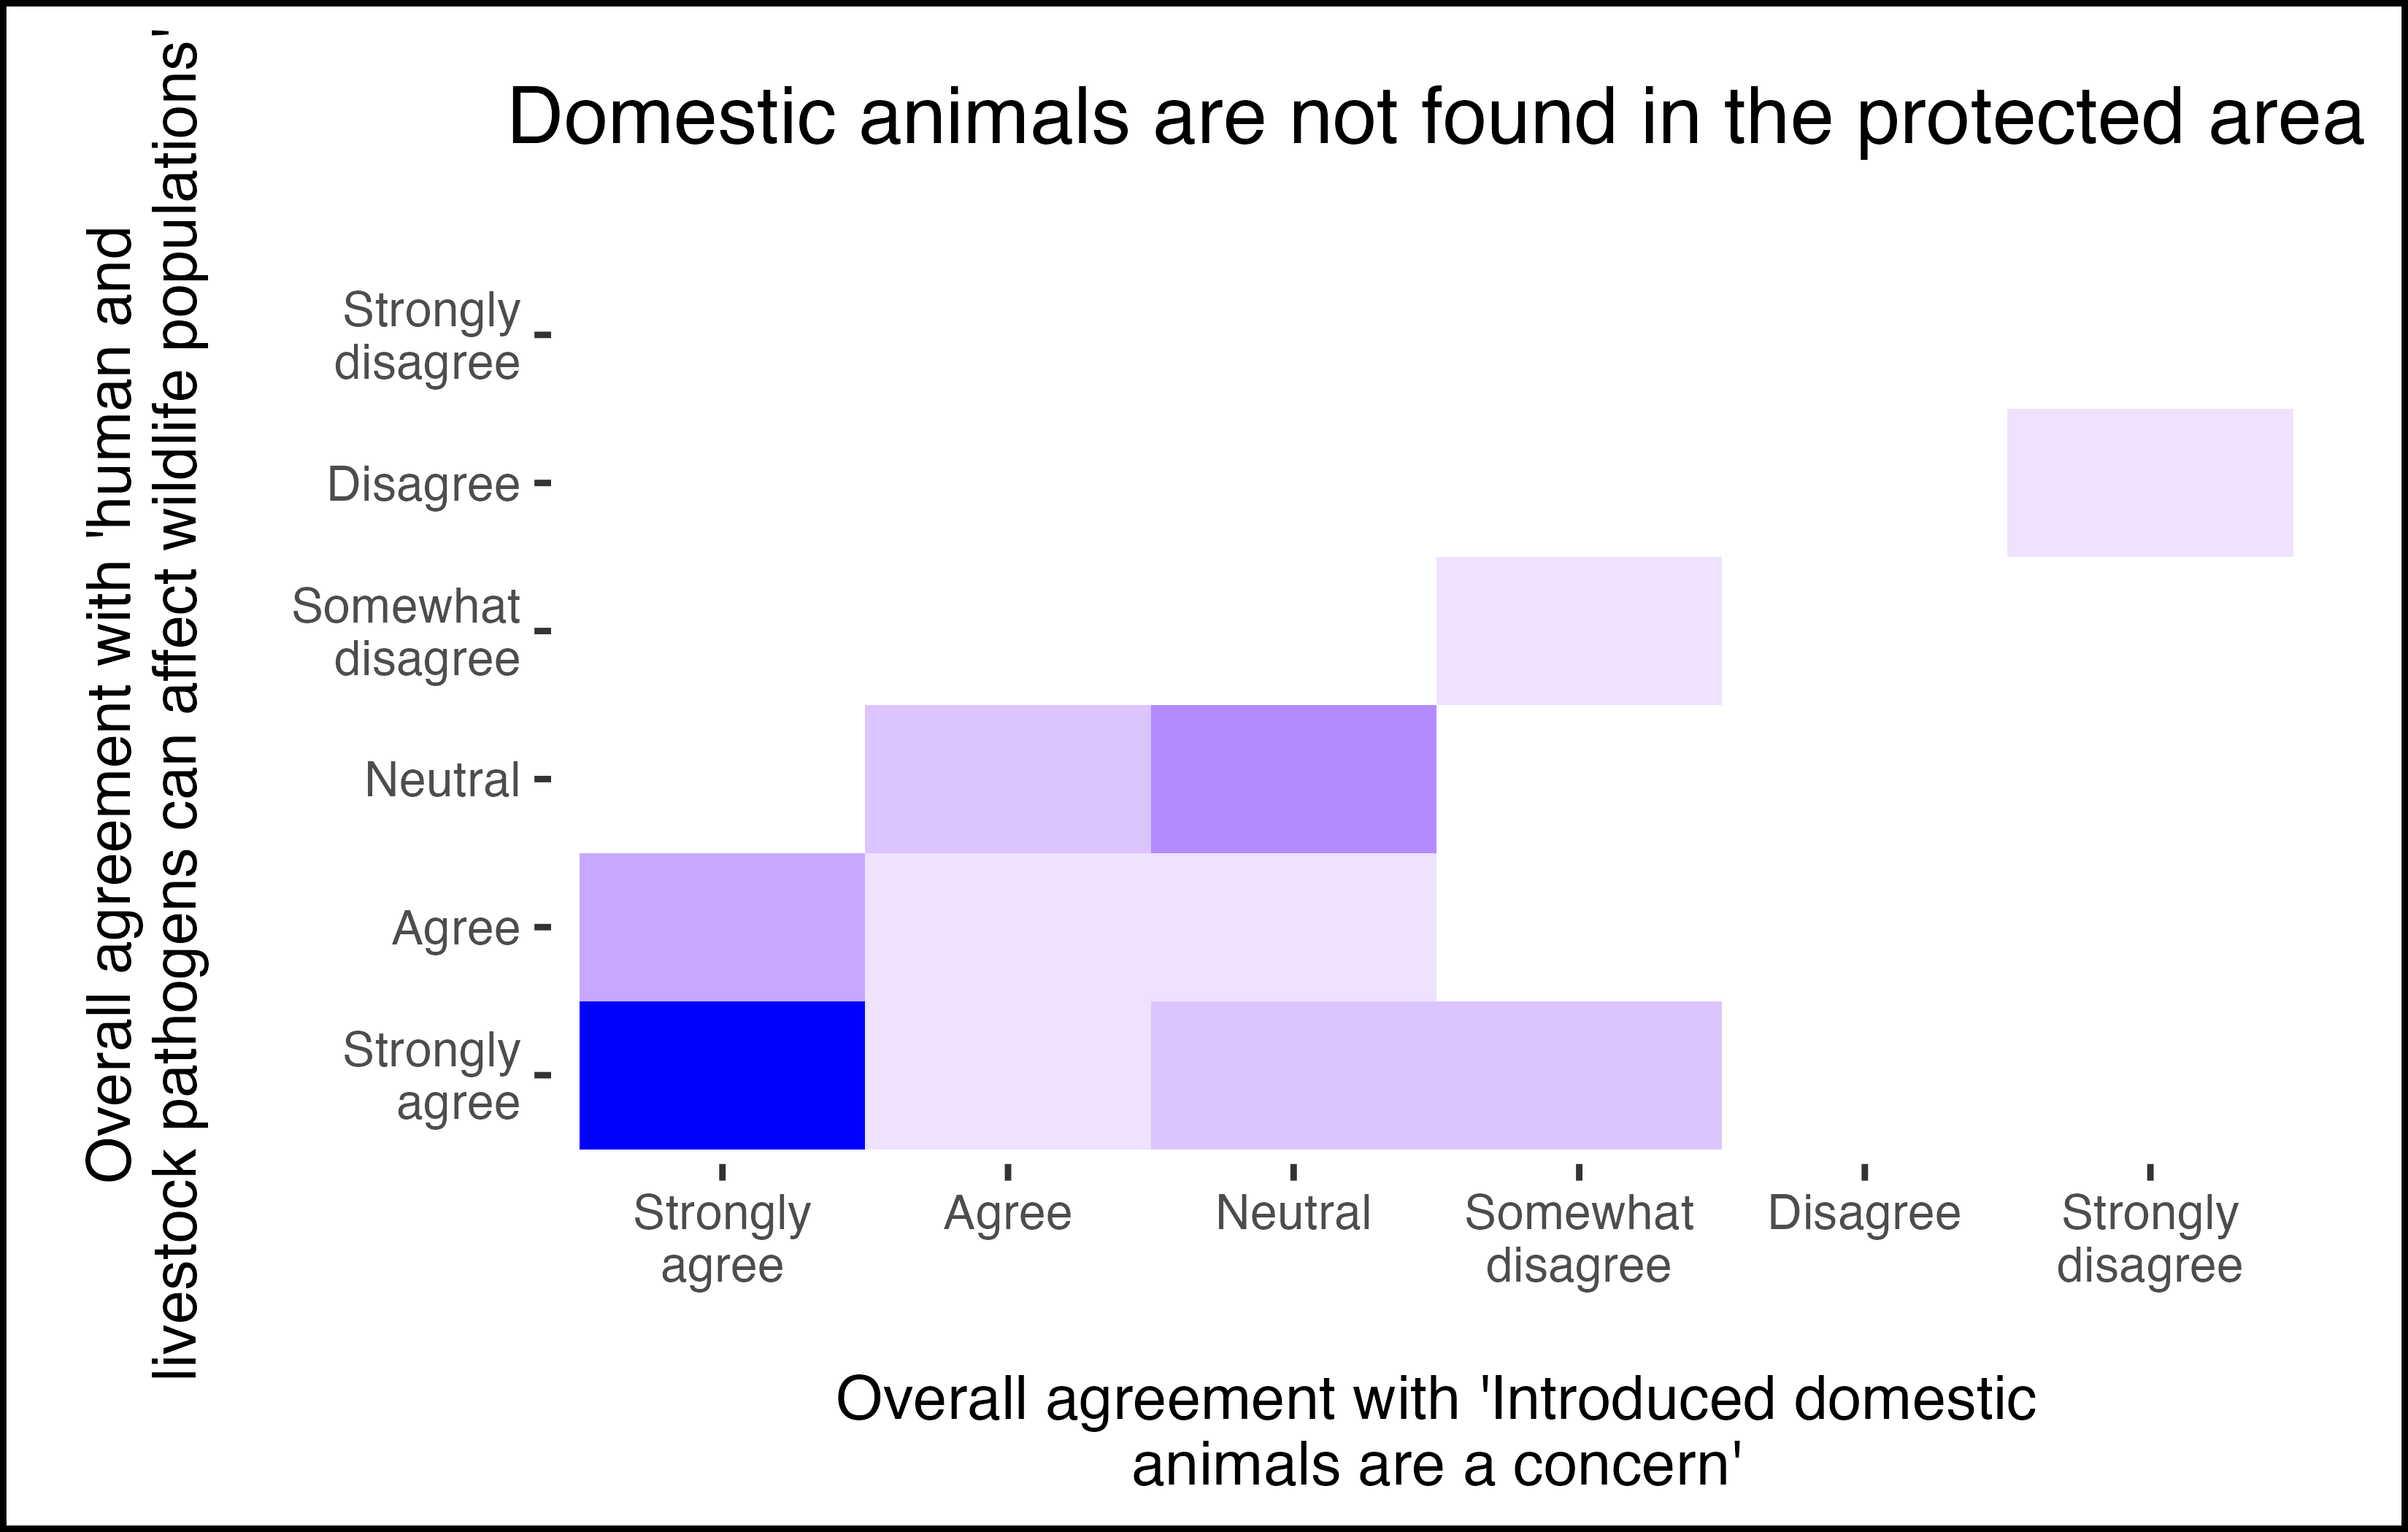
\includegraphics[width=5.20833in,height=\textheight]{plots/appedix_plot_5.png}

}

\end{figure}

\newpage

\hypertarget{appendix-s7.-distribution-of-protected-area-data-managers-responses-local-and-non-local-across-their-overall-agreement-with-human-and-livestock-pathogens-can-impact-wildlife-health-and-introduced-domestic-animals-are-a-concern-for-the-conservation-goals-of-the-protected-area-for-those-protected-area-data-managers-that-reported-the-presence-of-domestic-animals-in-the-protected-area.}{%
\paragraph{Appendix S7. Distribution of protected area data managers
responses (local and non-local) across their overall agreement with
``Human and livestock pathogens can impact wildlife health'' and
``Introduced domestic animals are a concern for the conservation goals
of the protected area'' for those protected area data managers that
reported the presence of domestic animals in the protected
area.}\label{appendix-s7.-distribution-of-protected-area-data-managers-responses-local-and-non-local-across-their-overall-agreement-with-human-and-livestock-pathogens-can-impact-wildlife-health-and-introduced-domestic-animals-are-a-concern-for-the-conservation-goals-of-the-protected-area-for-those-protected-area-data-managers-that-reported-the-presence-of-domestic-animals-in-the-protected-area.}}

\begin{figure}[H]

{\centering 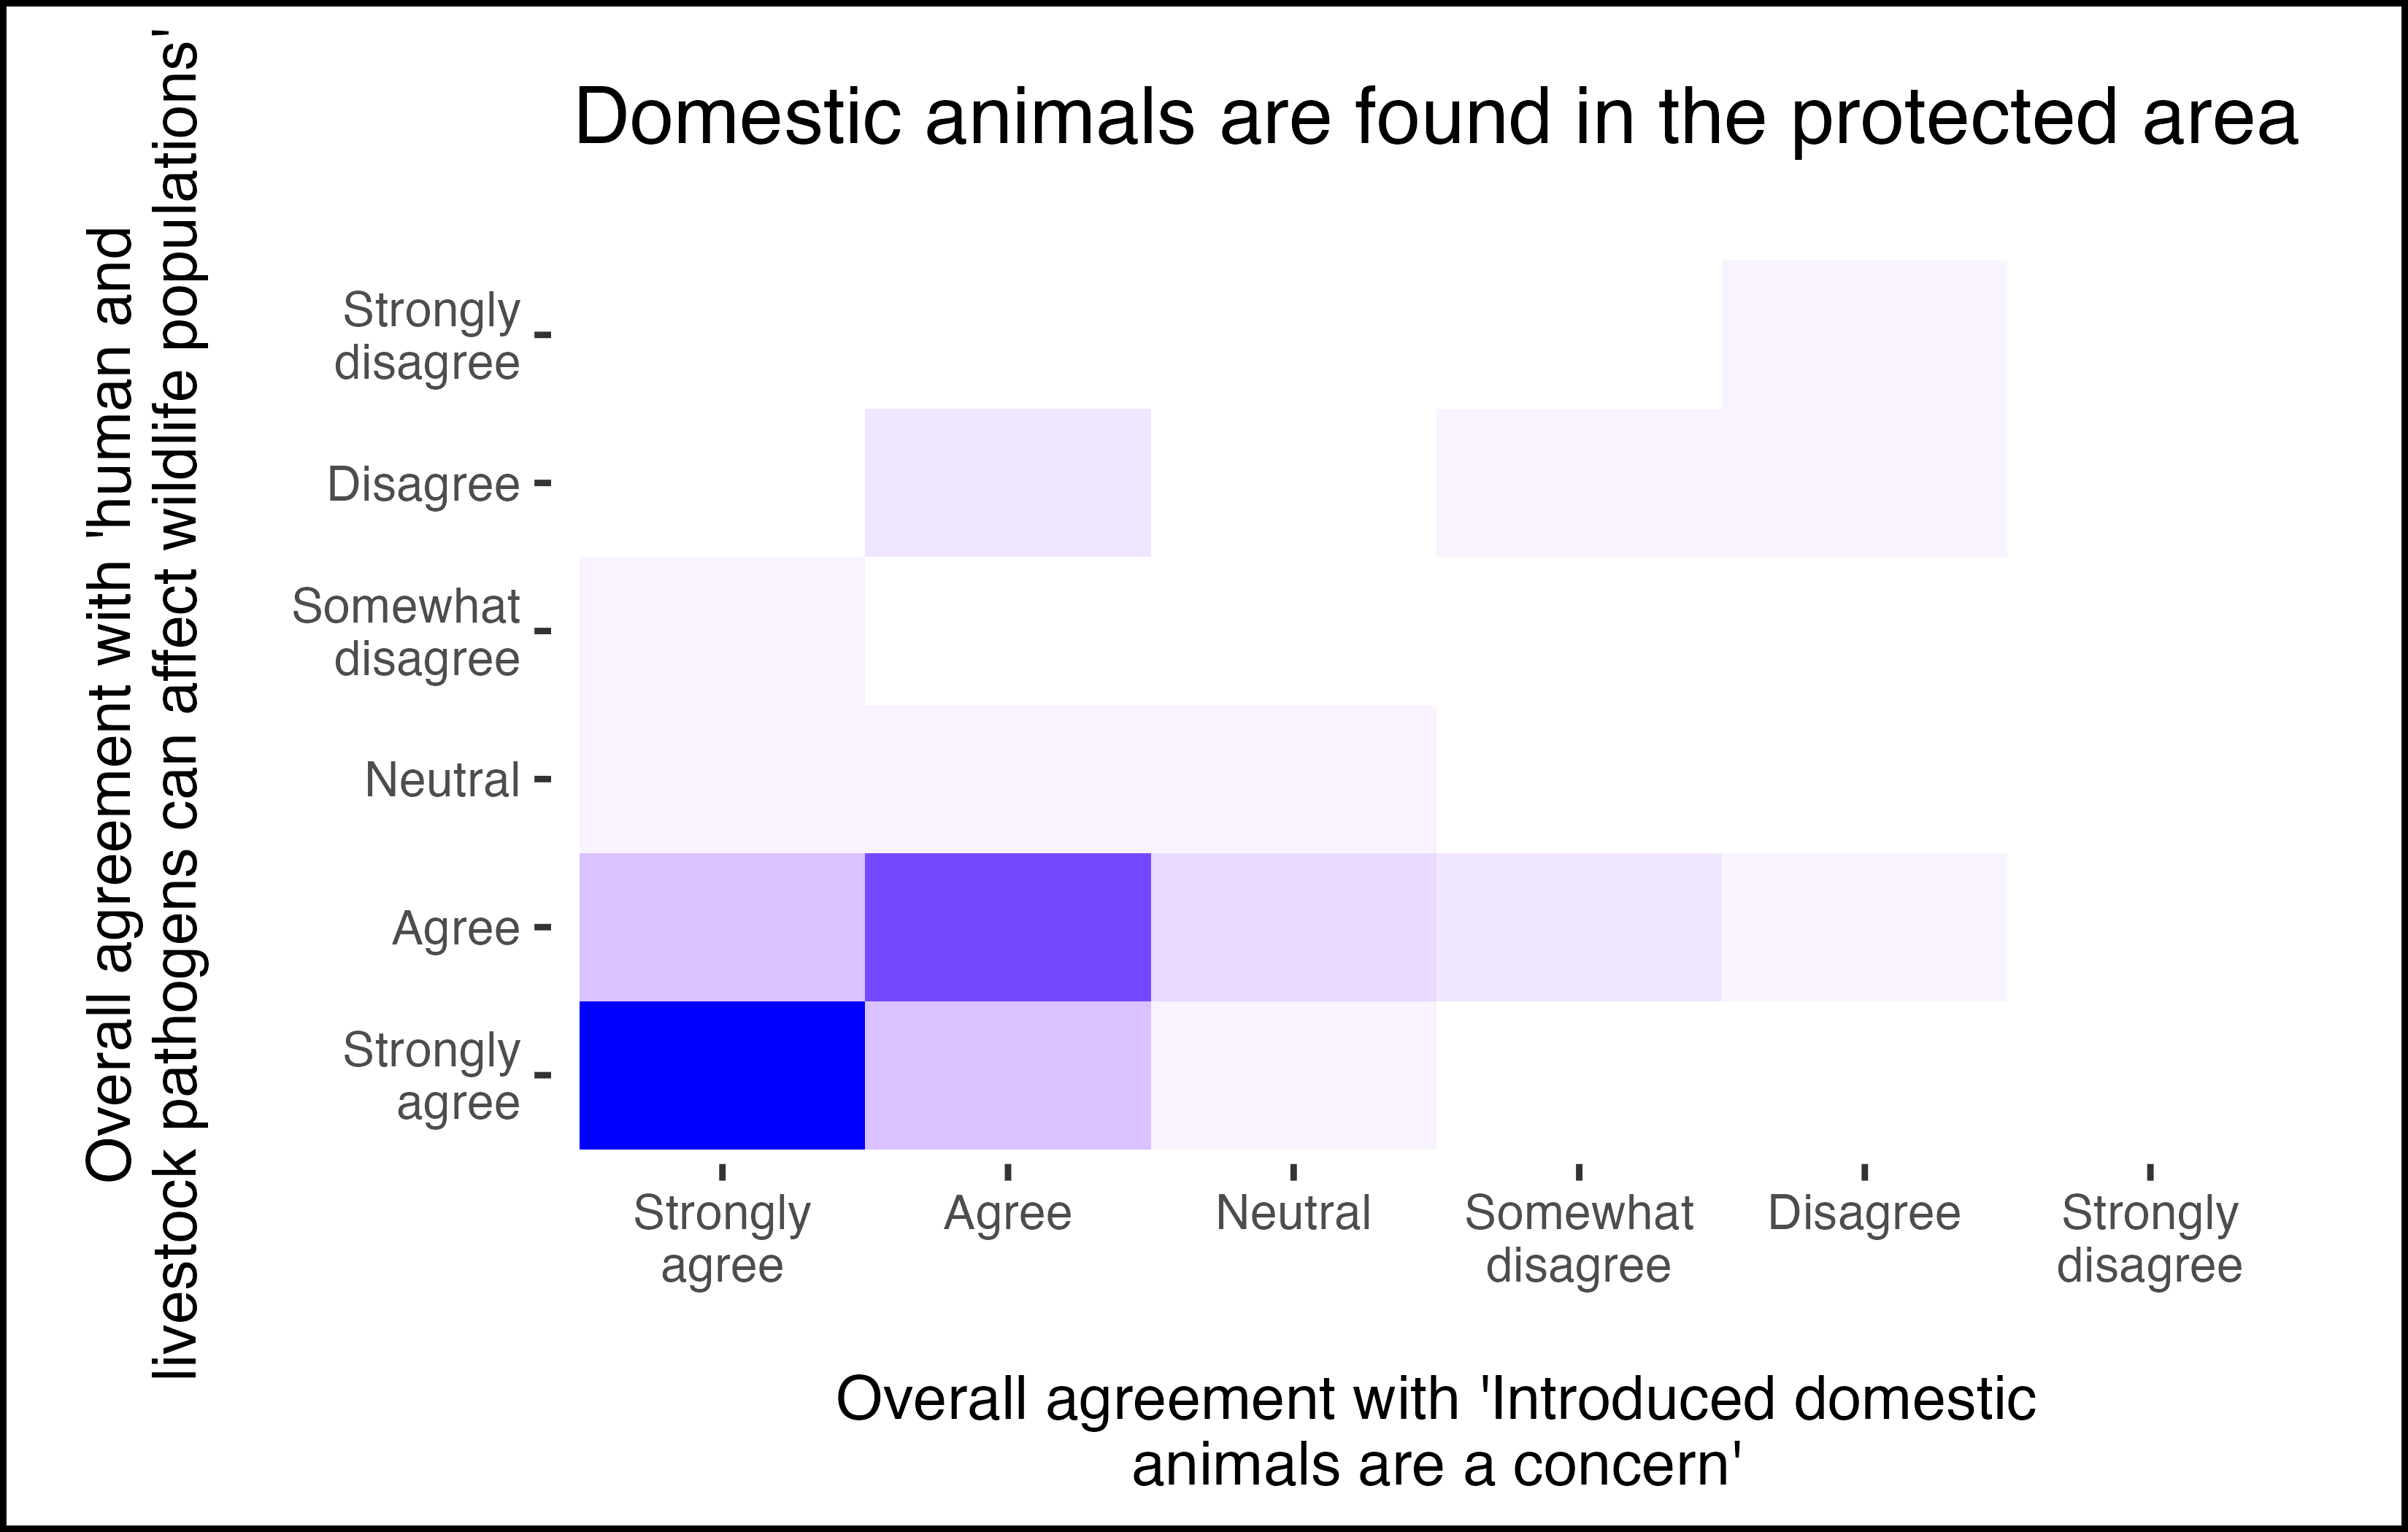
\includegraphics[width=5.20833in,height=\textheight]{plots/appedix_plot_6.png}

}

\end{figure}



\end{document}
